\documentclass[10pt]{article}
\usepackage{icmlko}

\icmlmeta{IP 파운데이션 월드모델}{47}{두 번의 승리는 같은 자리에서 나왔다}{구간을 통과한 배선 결정이 둘인데 둘 다 타깃 폭이다 --- 그리고 둘 다 의미로 고른 것을 검정이 뒤집은 것이다}

\begin{document}

\twocolumn[
\icmlheader

\begin{abstract}
노트 46은 웹툰 타깃 폭을 연령 등급에서 태그 수로 바꿨는데, 변형 다섯 개 중
점추정 최댓값을 고른 것이라 자기 한계 항목에 ``잡음일 수 있다''고 적었다. 짝지은
붓스트랩으로 자가 감사했다. \textbf{채택이 지지된다} --- 차이 $+$0.0981,
95\% 구간 {[}$+$0.042, $+$0.120{]}, P($>$0)$=$0.995. 그리고 그 크기가 노트 34의
도서 배선($+$0.0939)과 거의 같다. \textbf{지금까지 구간을 통과한 배선 결정이
둘인데 둘 다 타깃 폭 슬롯이고, 둘 다 의미로 맞아 보이는 것을 검정이 뒤집은
것이다} --- 도서에서는 장르 수 대신 판형, 웹툰에서는 연령 등급 대신 태그 수.
여섯 도메인에서 후보 예순 개를 다시 훑었다. 문턱(0.02)을 넘는 것이 하나 나왔고
(웹툰 굿즈 규모 $=$ 작가 수, $+$0.0355) 짝지은 구간을 붙이니
{[}$-$0.0027, $+$0.0741{]}로 아슬아슬하게 0을 포함해 \textbf{보류}했다.
P($>$0)$=$0.965다. 수집 쪽에서 결함도 하나 잡았다 --- 웹툰 418건이 \textbf{전부
연재 중}이고 완결작이 한 건도 없었다. 요일별 목록만으로 후보 상한에 닿아 완결
목록을 조회조차 하지 않은 것이다. 절반씩 뽑도록 고쳤다.
\end{abstract}
]

\section{자기 감사부터}

노트 46은 웹툰 타깃 폭 배선을 다섯 변형 중 점추정 최댓값으로 골랐다. 그 노트의
한계 항목에 이렇게 적었다 --- ``웹툰 배선 변형 다섯 개에서 최댓값을 골랐다.
짝지은 구간을 붙이지 않았다.''

붙였다.

\begin{table}[t]
\centering\tsize
\caption{웹툰 타깃 폭: 연령 등급 $\to$ 태그 수.}
\begin{tabular}{lr}
\toprule
점추정 & $+$0.1942 $\to$ $+$0.2923 \\
차이 & $+$0.0981 \\
짝지은 95\% 구간 & $[+0.042,\ +0.120]$ \\
P($>$0) & 0.995 \\
\midrule
판정 & \textbf{채택 지지} \\
\bottomrule
\end{tabular}
\end{table}

\section{두 승리가 같은 자리에 있다}

\begin{figure}[t]
\centering
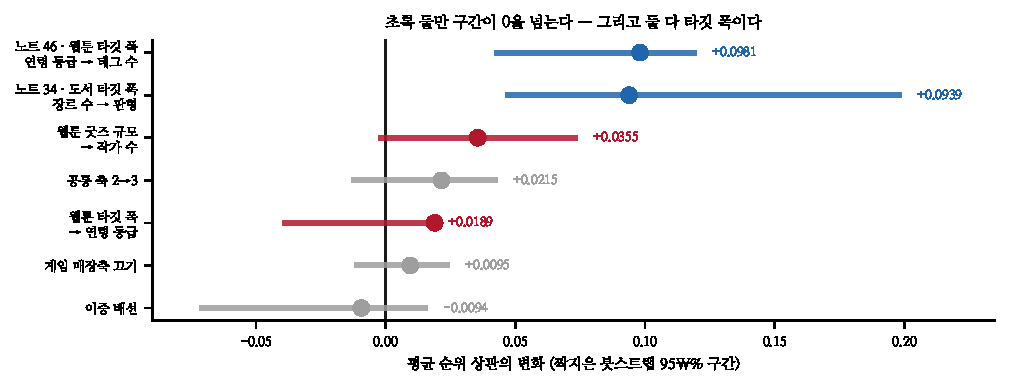
\includegraphics[width=\textwidth]{figs/wins.pdf}
\caption{지금까지 검정한 결정 전부. 초록만 구간이 0을 넘는다.}
\end{figure}

\begin{table}[t]
\centering\tsize
\caption{구간을 통과한 결정 둘.}
\begin{tabular}{llrl}
\toprule
노트 & 도메인 · 슬롯 & 차이 & 바꾼 내용 \\
\midrule
34 & 도서 · 타깃 폭 & $+$0.0939 & 장르 수 $\to$ 판형 \\
46 & 웹툰 · 타깃 폭 & $+$0.0981 & 연령 등급 $\to$ 태그 수 \\
\bottomrule
\end{tabular}
\end{table}

효과 크기가 4\% 차이로 거의 같다. 그리고 셋이 겹친다.

\begin{itemize}[leftmargin=1.1em,itemsep=0.15em]
\item \textbf{같은 슬롯} --- 둘 다 타깃 폭이다.
\item \textbf{같은 실수} --- 둘 다 ``몇 명에게 닿을 수 있게 만들었나''를 직접
      표기하는 것처럼 보이는 변수를 넣었다. 도서는 장르 수, 웹툰은 연령 등급.
\item \textbf{같은 교정} --- 둘 다 개별 변수를 훑어 라벨과 실제로 상관되는 것을
      찾아 바꿨다.
\end{itemize}

\claimx{배선 급 효과는 타깃 폭 슬롯에 몰려 있고, 그 슬롯이 가장 자주 잘못
배선된다. 다른 네 슬롯에서 구간을 통과한 결정은 아직 없다.}{매장 노출도나 굿즈
규모에서 구간을 통과하는 결정이 나오면 이 편중은 우연이었던 것이다. 슬롯이
다섯이고 승리가 둘이므로 우연히 같은 자리일 확률이 20\%다.}

\paragraph{왜 타깃 폭인가}
추측이지만 적어 둔다. 타깃 폭은 다섯 축 중 유일하게 \emph{상한}을 재는 축이다
--- 매장 노출도·입장 허들·굿즈 규모는 모두 정도의 문제인데 타깃 폭은 ``애초에
몇 명이 후보인가''를 잰다. 라벨이 사람 수인 도메인에서 그것이 가장 직접적인
제약이므로 효과가 크고, 동시에 ``의미로 그럴듯한'' 대리 변수가 가장 많아
잘못 배선되기도 쉽다.

\section{여섯 도메인에서 다시 훑는다}

웹툰 후보를 탐색 목록에 넣고 예순 개를 다시 쟀다.

\begin{figure}[t]
\centering
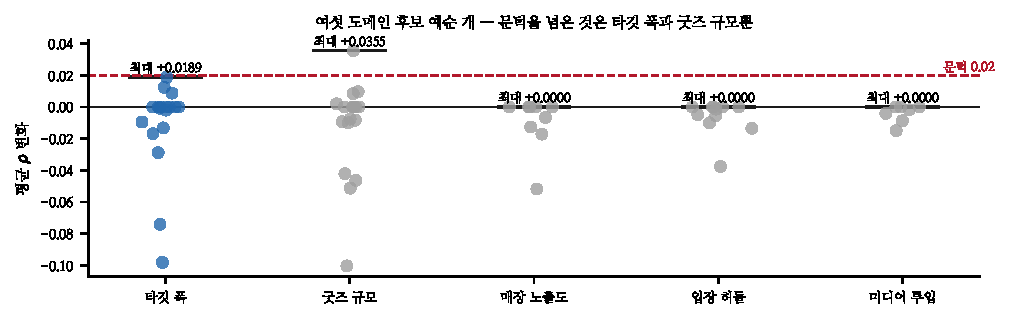
\includegraphics[width=\textwidth]{figs/slots.pdf}
\caption{슬롯별 후보 효과. 가로선이 각 슬롯의 최댓값이다.}
\end{figure}

\begin{table}[t]
\centering\tsize
\caption{상위 후보. 현행 6도메인 평균 $\rho=+0.2923$.}
\begin{tabular}{lllr}
\toprule
도메인 & 슬롯 & 후보 & $\Delta$ \\
\midrule
\textbf{웹툰} & \textbf{굿즈 규모} & \textbf{작가 수} & \textbf{$+$0.0355} \\
웹툰 & 타깃 폭 & 연령 등급(그대로) & $+$0.0189 \\
게임 & 타깃 폭 & 지원 언어 수 & $+$0.0124 \\
웹툰 & 굿즈 규모 & 회차 수 & $+$0.0097 \\
\bottomrule
\end{tabular}
\end{table}

문턱을 넘은 하나에 짝지은 구간을 붙였다.

\begin{table}[t]
\centering\tsize
\caption{보류한 둘.}
\begin{tabular}{lrrr}
\toprule
후보 & $\Delta$ & 95\% 구간 & P($>$0) \\
\midrule
웹툰 굿즈$=$작가 수 & $+$0.0355 & $[-0.003, +0.074]$ & 0.965 \\
웹툰 타깃폭$=$연령 등급 & $+$0.0189 & $[-0.040, +0.018]$ & 0.620 \\
\bottomrule
\end{tabular}
\end{table}

작가 수는 P$=$0.965로 아슬아슬하지만 구간이 0을 포함한다. 후보 예순 개 중
최댓값을 고른 것이므로 다중 비교까지 감안하면 더 보수적이어야 한다.
\textbf{보류하고 표본이 늘면 다시 본다.}

\paragraph{연령 등급 후보의 붓스트랩 편향}
타깃 폭을 연령 등급으로 되돌리는 후보는 점추정이 $+$0.0189인데 구간 상한이
$+$0.0181로 \emph{점추정보다 낮다}. 붓스트랩 분포가 한쪽으로 치우쳤다는 뜻이며,
점추정만 보고 판단하면 안 되는 이유를 그대로 보여 준다.

\section{수집 결함 하나}

웹툰 418건을 다시 보니 \textbf{완결작이 한 건도 없었다.} 연도 분포도
2024년 이후가 303건이다.

원인은 후보 수집 순서였다. 요일별 연재작을 먼저 다 모으고 남으면 완결작을
채우게 했는데, 요일 목록 일곱 개만으로 후보 상한에 닿아 완결 목록을 조회조차
하지 않았다. 관심 수는 연재 시작부터 쌓이므로 연재 중인 작품만 있으면 경과시간
편향이 그대로 남는다.

절반씩 뽑도록 고치고 다시 돌리고 있다. 노트 46의 한계 항목에 적어 둔 것이
실제로 결함이었다.

\begin{quote}\fontsize{9.5}{11.5}\selectfont
표본을 만들 때 \textbf{상한이 어느 경로에서 걸리는지} 봐야 한다. 두 경로에서
후보를 모으면서 앞쪽만으로 상한에 닿으면 뒤쪽은 없는 것과 같다. 필터가 무시되는
것(노트 22의 스팀 날짜, 노트 40의 텀블벅 창작자)과 같은 종류의 조용한 실패다.
\end{quote}

\section{한계}

\begin{itemize}[leftmargin=1.1em,itemsep=0.15em]
\item 슬롯 다섯에 승리 둘이므로 ``같은 자리''가 우연일 확률이 20\%다. 셋째
      승리가 나와야 패턴이라 부를 수 있다.
\item 웹툰 표본이 아직 연재작뿐이다. 완결작이 들어오면 배선 순위가 바뀔 수 있다.
\item 후보 예순 개 중 최댓값에 구간을 붙였다. 다중 비교 보정을 하지 않았다.
\item 짝지은 붓스트랩 200회다. 구간 끝점이 $\pm$0.01쯤 흔들린다.
\item 노트 34의 도서 배선 구간은 5도메인 시절 값이고 웹툰 것은 6도메인이다.
      같은 조건에서 다시 재지 않았다.
\end{itemize}

\section{다음}

\begin{enumerate}[leftmargin=1.3em,itemsep=0.15em]
\item 웹툰 완결작 확보 후 배선 재검정 --- 작가 수 후보가 살아나는지.
\item 나머지 네 도메인의 타깃 폭을 다시 훑는다. 승리가 그 자리에 몰려 있다면
      아직 안 본 후보가 있을 수 있다.
\item 노트 34의 도서 배선을 6도메인 조건에서 다시 재 같은 눈금으로 비교한다.
\item 다중 비교 보정 --- 후보가 예순 개인데 문턱 하나로만 걸렀다.
\end{enumerate}

\vspace{0.6em}
\hrule height 0.3pt
\vspace{0.5em}
{\footnotesize
\textbf{참고문헌}\\[0.3em]
Efron, B., Tibshirani, R. J. (1993). \emph{An Introduction to the Bootstrap}.
Chapman \& Hall.\\[0.15em]
Benjamini, Y., Hochberg, Y. (1995). Controlling the false discovery rate.
\emph{JRSS B}, 57(1), 289--300.\\[0.15em]
Cawley, G. C., Talbot, N. L. C. (2010). On over-fitting in model selection and
subsequent selection bias in performance evaluation. \emph{JMLR}, 11, 2079--2107.\\[0.15em]
Kaufman, S., Rosset, S., Perlich, C. (2012). Leakage in data mining.
\emph{ACM TKDD}, 6(4), 1--21.\\[0.15em]
Ben-David, S. et al. (2010). A theory of learning from different domains.
\emph{Machine Learning}, 79(1--2), 151--175.
}

\end{document}
